\subsection{Serie 6}%
\label{sub:serie_6}

\paragraph{Aufgabe 1}%
\label{par:aufgabe_1}

Erklären Sie: in einem Spiel in strategischer Form kann ein Spieler $i$ nicht
mehr als eine schwach (bzw. strikt) dominante Strategie haben.

\subparagraph{Lösung}%

Siehe Definitionen \ref{def:schwache_dominanz} und \ref{def:strikt_dominante_strategie}.
Angenommen ein Spieler hätte zwei strikt dominante Strategien $s^1$ und $s^2$.
Dann müssten nach Definition die Auszahlungen von $s^1$ echt größer sein als alle anderen
Auszahlungen des Spielers, insbesondere auch die Auszahlungen von $s^2$.
Gleichzeitig müssten nach Definition die Auszahlungen von $s^2$ auch echt größer als alle
anderen Auszahlungen des Spielers sein, insbesondere auch die Auszahlungen von $s^1$.
Diese beiden Aussagen stehen jedoch im Widerspruch zueinander, daher kann ein Spieler
nicht mehr als strikt dominante Strategie haben.

Eine analoge Argumentation gilt für die schwache Dominanz.

\paragraph{Aufgabe 2}%
\label{par:aufgabe_2}

Betrachten Sie folgendes Spiel in extensiver Form:
\begin{center}
  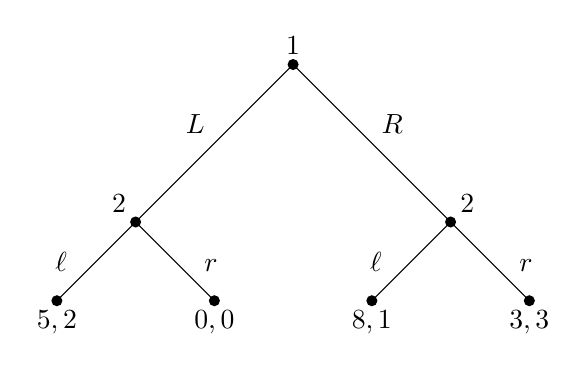
\begin{tikzpicture}
    \fill (0,0) circle (2pt) node [above] {$1$};
    \fill (-2,-2) circle (2pt) node [above left] {$2$};
    \fill (2,-2) circle (2pt) node [above right] {$2$};
    \fill (-3,-3) circle (2pt) node [below] {$5,2$};
    \fill (-1,-3) circle (2pt) node [below] {$0,0$};
    \fill (1,-3) circle (2pt) node [below] {$8,1$};
    \fill (3,-3) circle (2pt) node [below] {$3,3$};

    \draw (0,0) -- (-2,-2) node [midway,above left] {$L$};
    \draw (-2,-2) -- (-3,-3) node [near end,above left] {$\ell$};
    \draw (-2,-2) -- (-1,-3) node [near end,above right] {$r$};
    \draw (0,0) -- (2,-2) node [midway,above right] {$R$};
    \draw (2,-2) -- (1,-3) node [near end,above left] {$\ell$};
    \draw (2,-2) -- (3,-3) node [near end,above right] {$r$};
  \end{tikzpicture}
\end{center}

\begin{enumerate}
  \item Beschreiben Sie in Worten die Spielabfolge, potentielle Aktionen der Agenten und
    deren Informationen auf jeder Stufe.

  \item Erklären Sie den Unterschied zwischen einer Aktion und einer Strategie. Geben Sie
    für jeden Spieler ein Beispiel einer Aktion und ein Beispiel einer Strategie.

  \item Definieren Sie das Lösungskonzept Nash-GG (NGG). Was sind die reinen NGG dieses
    Spiels? Was sind die Ergebnisse dieser NGG?

  \item Definieren Sie ein Teilspiel und ein teilspielperfektes Nash-GG (SPNE) informell.
    Was sind die reinen SPNE dieses Spiels? Was sind die Ergebnisse dieser SPNE?

  \item Finden Sie das Konzept eines SPNE attraktiv? Ist es im Kontext dieses Spiels
    angemessen?
\end{enumerate}

\subparagraph{Lösung}%

\begin{enumerate}
  \item Anfangs ist Spieler 1 am Zug und entscheidet zwischen den möglichen Aktionen $L$
    und $R$.
    Danach ist Spieler 2 am Zug und weiß, ob Spieler 1 $L$ oder $R$ gespielt hat.
    Spieler 2 entscheidet, ob er $\ell$ oder $r$ spielt.

  \item Eine Aktion wird nur an einem Knoten im Spielbaum ausgeführt, während eine
    Strategie ein „Plan für alle Eventualitäten ist.“

    Spieler 1 hat z.\,B. die Aktion $L$ und auch die Strategie $L$.
    Spieler 2 hat z.\,B. die Aktion $\ell$ nachdem Spieler 1 $L$ gespielt hat
    und die Strategie $rr$.

  \item Ein Nash-Gleichgewicht ist eine Kombination von Strategien, wobei jeder Spieler
    genau eine Strategie wählt, von der aus es für keinen Spieler sinnvoll ist, von der
    gewählten Strategie als einziger abzuweichen.

    Zur Bestimmung der Nash-Gleichgewichte wird das extensive Spiel in ein statisches
    Spiel überführt:

    \begin{center}
      \begin{tabular}{cccccc}
        & & \multicolumn{4}{c}{Spieler 2}\\
        & & $\ell \ell$ & $\ell r$ & $r \ell$ & $rr$\\
        \cmidrule{3-6}
        \multirow{2}{*}{Spieler 1}
        & $L$ & $5,\underline{2}$ & $\underline{5},\underline{2}$ & $0,0$ & $0,0$\\
        \cmidrule{3-6}
        & $R$ & $\underline{8},1$ & $3,\underline{3}$ & $\underline{8},1$ &
        $\underline{3},\underline{3}$\\
        \cmidrule{3-6}
      \end{tabular}
    \end{center}

    Es gilt $\text{NGG} = \{(L, \ell r), (R, rr)\}$.

    Angenommen Spieler 2 entscheidet sich $rr$ zu spielen und kündigt dies offen für
    Spieler 1 an.
    Falls Spieler 1 $R$ spielt, erhält Spieler 2 die größtmögliche Auszahlung.
    Falls Spieler 1 jedoch $L$ spielt, dann erhält Spieler 2 die kleinstmögliche
    Auszahlung, obwohl Spieler 2 im linken Teilspiel durch die Aktion $\ell$ eine größere
    Auszahlung erhalten könnte.
    Die Ankündigung von Spieler 2 $rr$ zu spielen dient als \emph{Drohung} um Spieler 1 zu
    $R$ zu zwingen.
    Diese Drohung ist jedoch unglaubwürdig, weil es für Spieler 2 im linken Teilspiel
    rational wäre $\ell$ zu spielen.

  \item Ein Teilspiel ist ein Spiel, das in einem einzelnen Entscheidungsknoten des
    Spielbaums beginnt und alle Knoten enthält, die diesem Knoten nachfolgen, wobei keine
    Informationsbezirke getrennt werden dürfen.
    Ein Nash-Gleichgewicht ist \emph{teilspielperfekt}, wenn es ein Nash-Gleichgewicht in
    jedem Teilspiel induziert.

    In diesem Spiel gilt $\text{SPNE} = \{(L, \ell r)\}$.

  \item Ja und ja.
\end{enumerate}

\paragraph{Aufgabe 3}%
\label{par:aufgabe_3}

Betrachten Sie folgendes Spiel in extensiver Form:
\begin{center}
  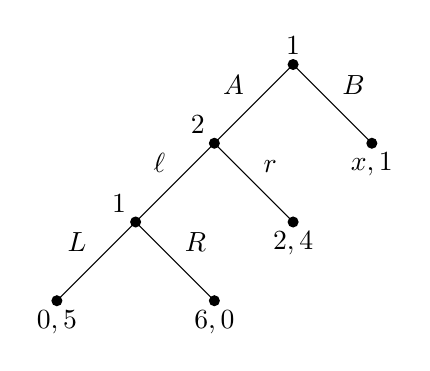
\begin{tikzpicture}
    \fill (0,0) circle (2pt) node [below] {$0,5$};
    \fill (2,0) circle (2pt) node [below] {$6,0$};
    \fill (1,1) circle (2pt) node [above left] {$1$};
    \fill (3,1) circle (2pt) node [below] {$2,4$};
    \fill (2,2) circle (2pt) node [above left] {$2$};
    \fill (4,2) circle (2pt) node [below] {$x,1$};
    \fill (3,3) circle (2pt) node [above] {$1$};

    \draw (3,3) -- (2,2) node [midway, above left] {$A$};
    \draw (3,3) -- (4,2) node [midway, above right] {$B$};
    \draw (2,2) -- (1,1) node [midway, above left] {$\ell$};
    \draw (2,2) -- (3,1) node [midway, above right] {$r$};
    \draw (1,1) -- (0,0) node [midway, above left] {$L$};
    \draw (1,1) -- (2,0) node [midway, above right] {$R$};
  \end{tikzpicture}
\end{center}

\begin{enumerate}
  \item Bestimmen Sie die Strategien der Spieler.
  \item Finden Sie die Menge der NGG dieses Spiels.
  \item Finden Sie die Menge der SPNE dieses Spiels für $x = 7,4,1$.
  \item Finden Sie das Konzept eines SPNE attraktiv?
    Vergleichen Sie die Situation für $x=7,4,1$.
\end{enumerate}

\subparagraph{Lösung}%

\begin{enumerate}
  \item Spieler 1 hat folgende Strategien: $AL, AR, BL, BR$.
    Spieler 2: $\ell, r$.

  \item Wir betrachten die Nash-Gleichgewichte für $x=7,4,1$ (auch wenn die
    Aufgabenstellung diese Werte für $x$ nicht vorgegeben hat):
    \begin{center}
      \begin{minipage}{0.30\textwidth}
        \begin{tabular}{cccc}
          & & \multicolumn{2}{c}{2}\\
          & $x=7$ & $\ell$ & $r$\\
          \multirow{4}{*}{1}
          & $AL$ & $0,\underline{5}$ & $2,4$\\
          & $AR$ & $6,0$ & $2,\underline{4}$\\
          & $BL$ & $\underline{x},\underline{1}$ & $\underline{x},\underline{1}$\\
          & $BR$ & $\underline{x},\underline{1}$ & $\underline{x},\underline{1}$
        \end{tabular}
      \end{minipage}
      \begin{minipage}{0.30\textwidth}
        \begin{tabular}{cccc}
          & & \multicolumn{2}{c}{2}\\
          & $x=4$ & $\ell$ & $r$\\
          \multirow{4}{*}{1}
          & $AL$ & $0,\underline{5}$ & $2,4$\\
          & $AR$ & $\underline{6},0$ & $2,\underline{4}$\\
          & $BL$ & $x,\underline{1}$ & $\underline{x},\underline{1}$\\
          & $BR$ & $x,\underline{1}$ & $\underline{x},\underline{1}$
        \end{tabular}
      \end{minipage}
      \begin{minipage}{0.30\textwidth}
        \begin{tabular}{cccc}
          & & \multicolumn{2}{c}{2}\\
          & $x=1$ & $\ell$ & $r$\\
          \multirow{4}{*}{1}
          & $AL$ & $0,\underline{5}$ & $\underline{2},4$\\
          & $AR$ & $\underline{6},0$ & $\underline{2},\underline{4}$\\
          & $BL$ & $x,\underline{1}$ & $x,\underline{1}$\\
          & $BR$ & $x,\underline{1}$ & $x,\underline{1}$
        \end{tabular}
      \end{minipage}
    \end{center}
    \begin{align*}
      \underset{x=7}{\text{NGG}} & = \{(BL, \ell), (BL, r), (BR, \ell), (BR, r)\}\\
      \underset{x=4}{\text{NGG}} & = \{(BL, r), (BR, r)\}\\
      \underset{x=1}{\text{NGG}} & = \{(AR, r)\}
    \end{align*}

  \item Per Rückwärtsinduktion ergeben sich folgende SPNE:
    \begin{align*}
      \underset{x \in \{4,7\}}{\text{SPNE}} & = \{(BR, r)\}\\
      \underset{x=1}{\text{SPNE}} & = \{(AR, r)\}
    \end{align*}
\end{enumerate}


\paragraph{Aufgabe 4}%
\label{par:aufgabe_4}

Betrachten Sie folgendes Spiel in extensiver Form:
\begin{center}
  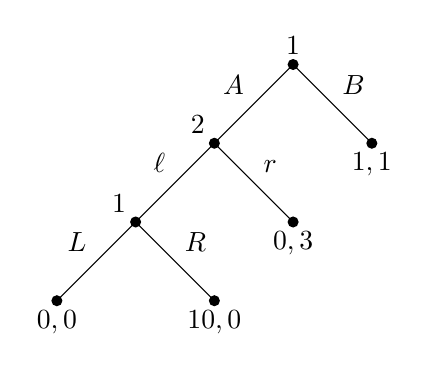
\begin{tikzpicture}
    \fill (0,0) circle (2pt) node [below] {$0,0$};
    \fill (2,0) circle (2pt) node [below] {$10,0$};
    \fill (1,1) circle (2pt) node [above left] {$1$};
    \fill (3,1) circle (2pt) node [below] {$0,3$};
    \fill (2,2) circle (2pt) node [above left] {$2$};
    \fill (4,2) circle (2pt) node [below] {$1,1$};
    \fill (3,3) circle (2pt) node [above] {$1$};

    \draw (3,3) -- (2,2) node [midway, above left] {$A$};
    \draw (3,3) -- (4,2) node [midway, above right] {$B$};
    \draw (2,2) -- (1,1) node [midway, above left] {$\ell$};
    \draw (2,2) -- (3,1) node [midway, above right] {$r$};
    \draw (1,1) -- (0,0) node [midway, above left] {$L$};
    \draw (1,1) -- (2,0) node [midway, above right] {$R$};
  \end{tikzpicture}
\end{center}

\begin{enumerate}
  \item Finden Sie die Menge NGG dieses Spiels.
  \item Finden Sie die Menge der SPNE dieses Spiels.
  \item Nehmen Sie nun an, dass Spieler 2 mit Wahrscheinlichkeit $\beta \in (0,1)$
    irrational ist und mit der selben Wahrscheinlichkeit $\ell, r$ wählt.
    Wie groß muss $\beta$ sein, damit es für Spieler $1$ optimal ist $A$ zu wählen?
\end{enumerate}

\subparagraph{Lösung}%

\begin{enumerate}
  \item Zur Bestimmung der NGG:
    \begin{center}
      \begin{tabular}{cccc}
        & & \multicolumn{2}{c}{2}\\
        & & $\ell$ & $r$\\
        \multirow{4}{*}{1}
        & $AL$ & $0,0$ & $0,\underline{3}$\\
        & $AR$ & $\underline{10},0$ & $0,\underline{3}$\\
        & $BL$ & $1,\underline{1}$ & $\underline{1},\underline{1}$\\
        & $BR$ & $1,\underline{1}$ & $\underline{1},\underline{1}$
      \end{tabular}
    \end{center}
    Damit gilt $\text{NGG} = \{(BL, r), (BR,r)\}$.

  \item Per Rückwärtsinduktion ergibt sich: $\text{SPNE} = \{(BR,r)\}$.

  \item Beim folgenden Teilspiel wählt Spieler 1 immer $R$, da Spieler 1 rational ist:
    \begin{center}
      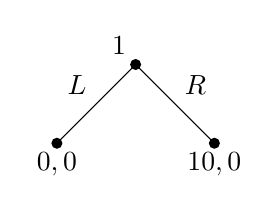
\begin{tikzpicture}
        \fill (0,0) circle (2pt) node [below] {$0,0$};
        \fill (2,0) circle (2pt) node [below] {$10,0$};
        \fill (1,1) circle (2pt) node [above left] {$1$};

        \draw (1,1) -- (0,0) node [midway, above left] {$L$};
        \draw (1,1) -- (2,0) node [midway, above right] {$R$};
      \end{tikzpicture}
    \end{center}
    Beim sich daraus ergebenden Teilspiel
    \begin{center}
      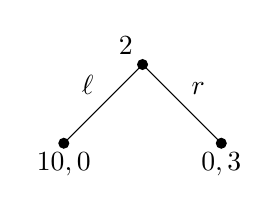
\begin{tikzpicture}
        \fill (1,1) circle (2pt) node [below] {$10,0$};
        \fill (3,1) circle (2pt) node [below] {$0,3$};
        \fill (2,2) circle (2pt) node [above left] {$2$};

        \draw (2,2) -- (1,1) node [midway, above left] {$\ell$};
        \draw (2,2) -- (3,1) node [midway, above right] {$r$};
      \end{tikzpicture}
    \end{center}
    ist Spieler 2 mit der Wahrscheinlichkeit $\beta$ irrational und wählt mit der
    Wahrscheinlichkeit $\frac{1}{2}$ entweder $\ell$ oder $r$.
    Daraus ergeben sich folgende Erwartungsnutzen:
    \begin{align*}
      EU_2 & = \beta(\frac{1}{2} \cdot 0 + \frac{1}{2} \cdot 3) + (1-\beta) \cdot 3
             = 3 - \frac{3}{2}\beta\\
      EU_1 & = \beta(\frac{1}{2} \cdot 10 + \frac{1}{2} \cdot 0) + (1-\beta) \cdot 0
             = 5 \beta
    \end{align*}
    Beim sich daraus ergebenden Teilspiel auf oberster Ebene
    \begin{center}
      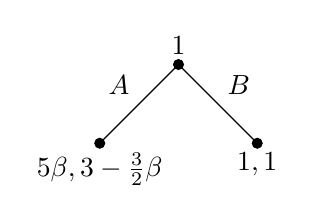
\begin{tikzpicture}
        \fill (2,2) circle (2pt) node [below] {$5\beta, 3-\frac{3}{2}\beta$};
        \fill (4,2) circle (2pt) node [below] {$1,1$};
        \fill (3,3) circle (2pt) node [above] {$1$};

        \draw (3,3) -- (2,2) node [midway, above left] {$A$};
        \draw (3,3) -- (4,2) node [midway, above right] {$B$};
      \end{tikzpicture}
    \end{center}
    fragt sich Spieler 1: für welches $\beta$ gilt $5\beta > 1$?
    Für $\beta > \frac{1}{5}$.
\end{enumerate}

\paragraph{Aufgabe 5}%
\label{par:aufgabe_5}

In einer Amerikanischen Fernsehshow wird den Spielern die Wahl zwischen dem Öffnen einer
von drei Türen (rot, grün, blau) angeboten.
Hinter einer Tür verbirgt sich ein Preis, hinter den anderen nichts.
Die Spieler haben keinen Grund anzunehmen, dass eine der Türen mit höherer
Wahrscheinlichkeit zu einem Preis führt als eine andere.
Der Quizmaster weiß, hinter welcher Tür der Preis liegt.
Nachdem ein Spieler eine der Türen gewählt (aber noch nicht geöffnet) hat, \emph{muss} der
Quizmaster eine der anderen Türen öffnen.
Der Spieler kann sich dann entscheiden, ob er bei der von ihm ursprünglich gewählten Tür
bleibt, oder ob er zu einer anderen Tür wechselt.
Nehmen Sie an, dass die Spieler die Wahrscheinlichkeit den Preis zu bekommen maximieren,
während der Quizmaster diese Wahrscheinlichkeit minimieren möchte.

\begin{enumerate}
  \item Beschreiben Sie eine optimale Strategie des Quizmasters.
    Nehmen Sie im Weiteren an, dass der Quizmaster diese Strategie verfolgt.

  \item Was sollte der Spieler tun, wenn er gefragt wird, ob er wechseln möchte?
    Begründen Sie Ihre Antwort.
\end{enumerate}
